% \begin{figure}[h]
%  \centering
%  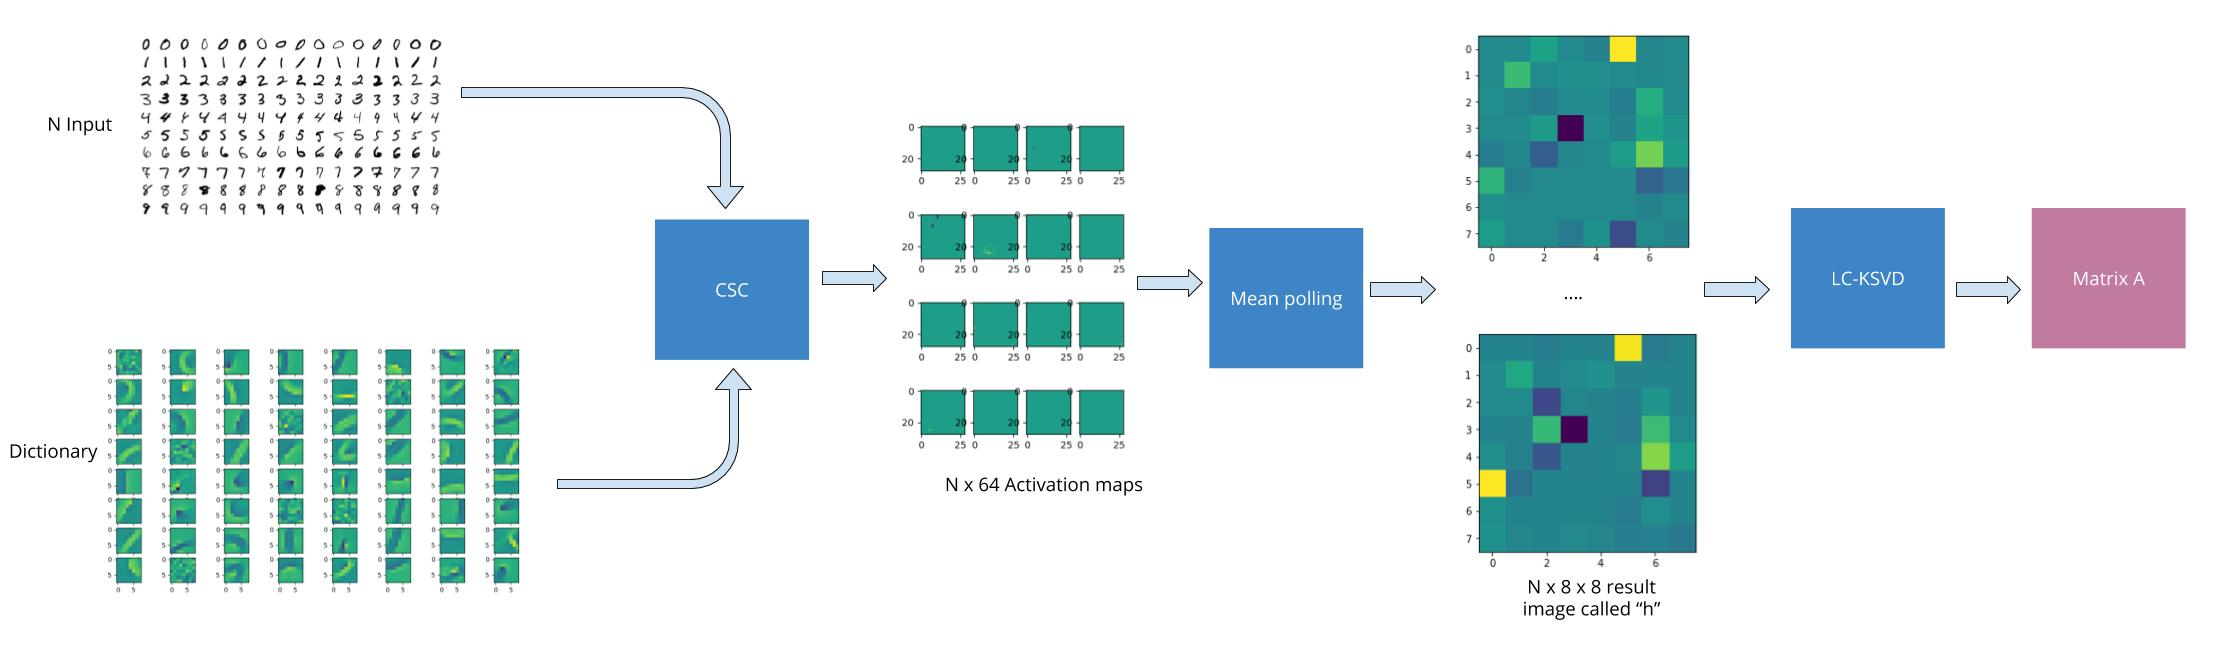
\includegraphics[scale=0.2]{Training_phase.jpg}
%  % Training phase.jpg: 2217x648 px, 72dpi, 78.21x22.86 cm, bb=0 0 2217 648
%  \caption{Training phase}
% \end{figure}
% \begin{figure}[h]
%  \centering
%  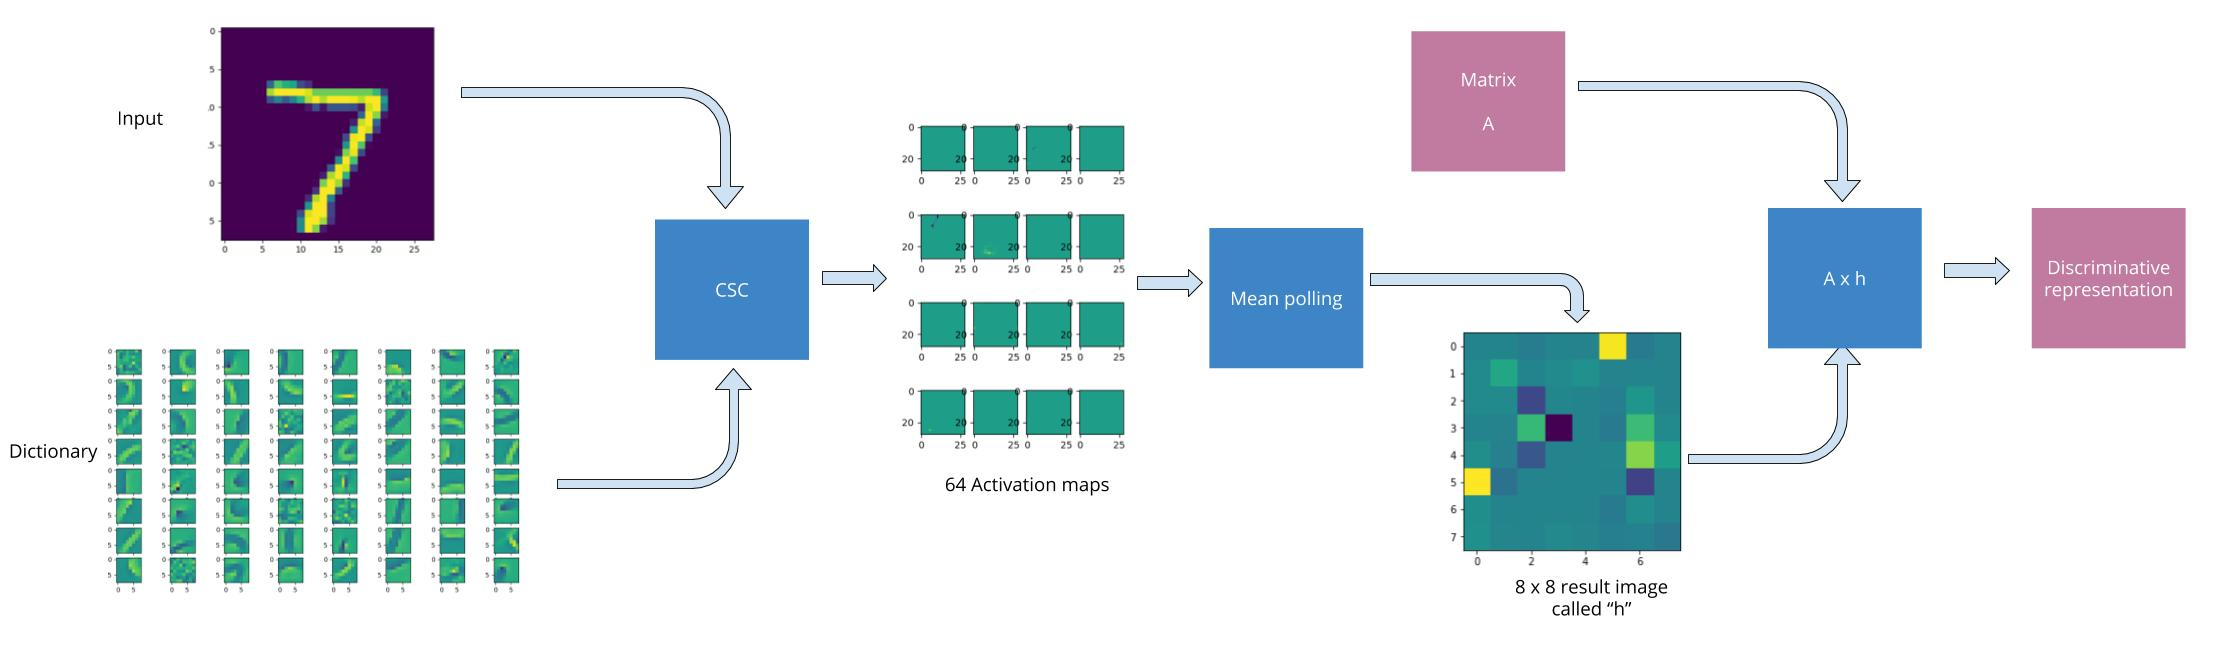
\includegraphics[scale=0.2]{Test_phase.jpg}
%  % Test phase.jpg: 2217x648 px, 72dpi, 78.21x22.86 cm, bb=0 0 2217 648
%  \caption{Test phase}
% \end{figure}
\section{ML-CSC}
In order to get a discriminative Convolutional Sparse Coding, \cite{DBLP:journals/corr/abs-1708-08705,8398588} proposed to extend the CSC model to a Multi-Layers version (called ML-CSC). Indeed,  adding a new CSC layer allows the algorithm to capture more complex patterns.\\
Add a new layer corresponds to get the features maps $Z$ obtained by CSC in the previous layers and use them like the input signal with a new dictionary, in other word $D_1$  (layer 1's dictionary) contain simple patterns, the convolution product $D_1 * D_2$ contains  a linear combination of atoms from $D_1$, merging them to create more complex patterns, called molecules. Mathematically,for $L$ layers:
\begin{center}
 $X = D_1 * Z_1$ \hspace{1cm} Layer 1\\
 $Z_1 = D_2 * Z_2$\hspace{1cm} Layer 2\\
 $Z_2 = D_3 * Z_3$\hspace{1cm} Layer 3\\
 \dots\\
 $Z_{L-1} = D_L * z_L$ \hspace{1cm} Layer L\\
 Then X can be rewriten by:\\
 $X = D_1 * D_2 * D_3 *\dots *D_L * z_L$
\end{center}
Then it is possible to rewrite the dictionary learning algorithm to extend it to a multi-layer version:\\
\begin{algorithm}
 \caption{Multi-Layer Convolutional Dictionary Learning}
 \begin{algorithmic}
  \REQUIRE Training sample $\{x_1, x_2, \dots, x_k \}$, initial convolutional dictionaries $\{D_1, D_2, \dots, D_L \}$, the number of iterations for gradient descent T
  \FOR{$k=1, \dots, k$}
        \STATE Sparse Coding: $z_L \leftarrow \underset{z_L}{\argmin} \|x_k - D_L z_L\|^2_2  + \lambda \|z_L\|_1$
        \STATE \textit{/* Update dictionaries*/}
        \FOR{$i = L, \dots, 1$}
            \FOR{$t = 1, \dots, T$}
                 \STATE $D_i \leftarrow \mathcal{H}[D_i - \alpha ((y_k -D_i Z_i)Z_i^T) ] $
            \ENDFOR
        \ENDFOR
        \FOR{$t = 1, \dots, T$}
            \STATE $D_1 \leftarrow D_i - \alpha ((y_k -D_iZ_1) Z_1^T)$
        \ENDFOR
  \ENDFOR
 \end{algorithmic}
\end{algorithm}\\
Note that $D_1$ is not updated with the others dictionaries $D_i$, this is because its imposed that the other dictionaries $D_i$ are sparse to be sure that the feature maps $Z_i$ are also sparse. This is possible by applying the hard-thresholding operation $\mathcal{H}$ on them.
\section{Tests details}
For all our experimentations on ML-CSC we used a matlab demo writen by 
Jeremias Sulam \footnote{\url{https://sites.google.com/view/jsulam/}} (writer of \cite{DBLP:journals/corr/abs-1708-08705,8398588}) that he provided us. We want to thank him for that.
\subsection{Application of ML-CSC on MNIST}
\begin{figure}[h]
 \centering
 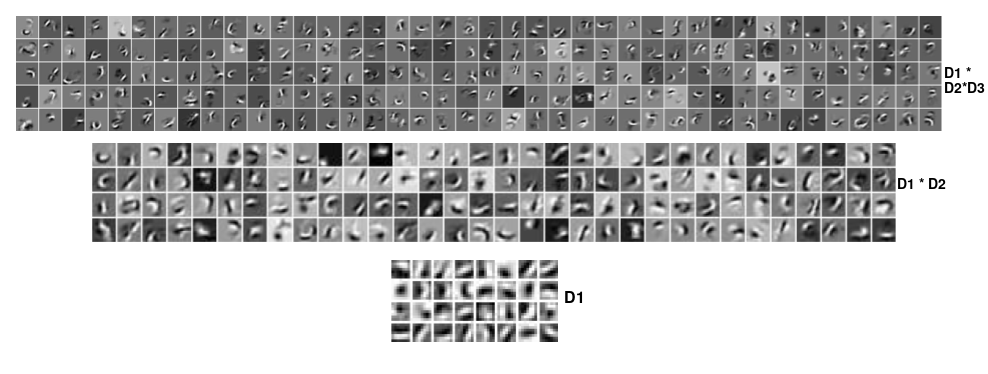
\includegraphics[scale=2]{Discriminative_CSC.png}
 % Discriminative CSC.png: 1001x266 px, 72dpi, 35.31x9.38 cm, bb=0 0 1001 266
 \caption{Dictionary's atoms at each layer}
 \label{fig:DCSC}
\end{figure}
\begin{figure}[h]
 \centering
 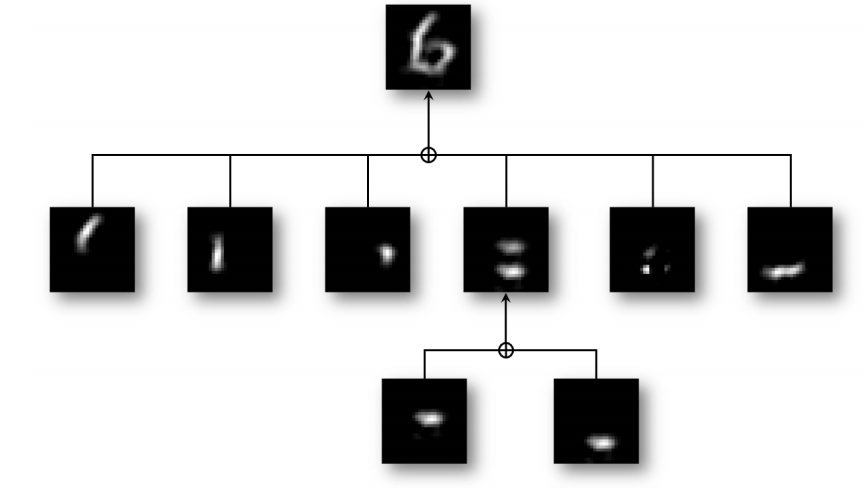
\includegraphics[scale=0.3]{decomp.png}
 % decomp.png: 864x488 px, 96dpi, 22.86x12.91 cm, bb=0 0 648 366
 \caption{From atoms to molecules: Illustration of the ML-CSC
model for a number 6. Two local convolutional atoms (bottom
row) are combined to create slightly more complex structures
– molecules – at the second level, which are then combined
to create the global atom representing, in this case, a digit \cite{DBLP:journals/corr/abs-1708-08705}}
 \label{fig:decomp}
\end{figure}

Here we see in figure \ref{fig:DCSC}the 3 layers of dictionaries with the learned forms. The deeper the dictionary got the more complex forms and therefore discriminative. In the figure \ref{fig:decomp} a reconstruction of a 6 is displayed. 

\subsection{Classification for ML-CSC}

With the Multi-layer Convolutional Sparse Coding, if we try to classify the obtained features we got:
\begin{itemize}
 \item SVM Accuracy = 93,67\%
 \item K-means Accuracy = 11,46\%
\end{itemize}
The problem here is that once again, we get bad results for K-means because the representations for the same classes can be different and the only way to solve it is to use the information of the labels that we have in the supervised setting. To address this problem we proposed a new method based on LC-KSVD.
\newpage
\section{LC-ML-CSC}
SAs we used Label-Consistent Sparse Coding instead of traditional Sparse Coding to get more discriminating Sparse coefficients, we want to create a new convolutional Multi-Layer Sparse Coding model that adds a consistent Label term: We called it \textit{Label Consistent Multi-Layer Convolutional Sparse coding} (LC-ML CSC).\\
We already explained what is the label consistent term and the multi-layers convolutional Sparse Coding, thus we can already present the LC-ML CSC algorithm:
\begin{algorithm}
\caption{Labels Consistent Multi Layers Convolutional Sparse Coding (LC-MLCSC )}
\begin{algorithmic} 
\REQUIRE Y: input data, Q: discriminative matrix
\FOR{$k = 1,\dots,K$} 
    \STATE $y_k \leftarrow $ The $k^{th}$ batch of Y
    \STATE \textit{/* Sparse Coding */} 
    \STATE $z_{kL} = \underset{z_k}{\argmin} \underset{CSC\ normal}{\underbrace{\|y_k - D^L z_k\|^2_2 +\alpha \|z_k\|_1}} + \underset{LC composant}{\underbrace{\beta \|Q -A z_k\|}}$ 
    \STATE $ = z_k  - \alpha(D^T (Dz_k -y_k) + \lambda(sign(z_k)) + \beta (A^T(A z_k -Q)))$
    \STATE \textit{/* Dictionary Update */}
    \FOR{$i=L, \dots, L $}
        \STATE $D_i \leftarrow \mathcal{H}[D_i - \alpha ((y_k -D_iz_k)z_k^T) ] $
    \ENDFOR
    \STATE \textit{/* Update Matrix A */}
    \STATE $A \leftarrow A + \alpha (\beta (Q-Az_k)z_k^T)$
\ENDFOR
\RETURN $z_k$, D, A
\end{algorithmic}
\end{algorithm}
% \begin{algorithm}
% \caption{Labels Consistant Multi Layers Convolutional Sparse Coding 2(LC-MLCSC 2)}
% \begin{algorithmic} 
% \REQUIRE Y, Q
% \FOR{$k = 1,\dots,K$} 
%     \STATE $y_k \leftarrow $ Le $k^{eime}$ batch de Y
%     \STATE Sparse Coding: 
% \STATE Sparse Coding: $z_L \leftarrow \underset{z_L}{\argmin} \|x_k - D_L z_L\|^2_2  + \lambda \|z_L\|_1$
%     \STATE Dictionary Update:
%     \FOR{$i=L, \dots, L $}
%         \STATE $D_i \leftarrow \mathcal{H}[D_i - \alpha ((y_k -D_iz_k)z_k^T) ] $
%     \ENDFOR
%     \STATE Mise à jour de la matrice A:
%     \STATE $A \leftarrow A + \alpha (\beta (Q-Az_k)z_k^T)$
% \ENDFOR
% \RETURN $z_k$, D, A
% \end{algorithmic}
% \end{algorithm}

However, at the moment when we write these internship report the LC-ML CSC still a work in progress method. And we don't have a good result in classifying even with SVM. That why we will not present the results of this method here.
